\chapter{Experiments}
\label{sec:unchapitre}
\minitoc


%\noindent Chapeau introductif
%\begin{itemize}
%	\item Application sur des bases de séries temporelles univariés de la littérature (Keogh)
%	\item Données Schneider? ou Expliquer les problématiques de Schneider
%\end{itemize}
\fbox{  \parbox{0.9\textwidth}{
		In this chapter, we evaluate the efficiency of our proposed algorithm {\sc m}$^2${\sc tml} on public datasets for classification problems of univariate time series. \\
		First, we describe the datasets. Secondly, we detail the experimental protocol. Finally, we present and discuss the obtained results.
	}  }
%-----------------------------------------------------------------------------
\section{Description}
The efficiency of the  learned multi-modal and multi-scale dissimilarities $D$ and $D_{\mathcal{H}}$ is evaluated through  a $1-$NN classification on 30 public datasets \footnote{PowerCons:   \url{https://archive.ics.uci.edu/ml/datasets/Individual+household+electric+power+consumption}, {\sc bme} and {\sc umd}:  \url{http://ama.liglab.fr/~douzal/tools.html}.} \cite{Keogh2011}. The considered data encompass time series that involve global or local temporal differences, require or not time warping, with  linearly or non linearly separable  neighborhoods. Table \ref{tab:DatasetDescription} gives a description of the datasets considered for our experiments and Fig. \ref{fig:dataset} gives the temporal representation of some of them. The learnt metrics $D$ and $D_{\mathcal{H}}$ are compared to five alternative uni-modal metrics covering: 
\begin{enumerate}
	\item The  standard  Euclidean distance and dynamic time warping referenced as $d_A$ (Eq. \ref{eq:A}) and  {\sc dtw}
	\item The behavior-based measures  $d_B$ (Eq. \ref{eq:B}) and $d_{B-\mbox{\sc dtw}}$ its counterpart  for asynchronous time series, that is $d_B$ is evaluated once time series synchronized by dynamic programing
	\item The frequential-based metric  $d_F$ (Eq. \ref{eq:F}). 
\end{enumerate}
The alternative  metrics are evaluated  as usual by involving the all time series elements ({\it i.e.} at the global scale). For  $D$ and $D_{\mathcal{H}}$, we consider a 21-dimensional embedding space  $\mathcal{E}$ that relies, for synchronous (resp. asynchronous) data,  on 3 log-normalized dissimilarities $d_{A}^{s}$, $d_{B}^{s}$ (resp. {\sc dtw}$^{s}$, $d_{B-\mbox{\sc dtw}}^{s}$), and $d_{F}^{s}$, at 7 temporal granularities $s \in \{0,...,6\}$ obtained by binary segmentation as described in Section \ref{sec:multiscale}. \\

\begin{table}[h!]
	\small
	\begin{center}
		\renewcommand{\arraystretch}{1}
		\resizebox{0.7\textwidth}{!}{
			\begin{tabular}{lcccc}
				\hline
				Dataset    	& Nb. Class & Nb. Train 
				& Nb. Test  & TS length\\
				\hline
				Trace 				& 4 & 100 & 100  & 275 \\
				CBF 				& 3 & 30  & 900  & 128 \\
				CC					& 6 & 300 & 300  & 60  \\
				UMDsmooth 			& 3 & 360 & 1440 & 150 \\
				BMEsmooth 			& 3 & 300 & 1500 & 128 \\
				DiatomSizeReduc 	& 4 & 16  & 306  & 345 \\
				ItalyPowerDemand 	& 2 & 67  & 1029 & 24  \\
				Symbols 			& 6 & 25  & 995  & 398 \\
				GunPoint			& 2 & 50  & 150  & 150 \\
				FacesUCR			& 14& 200 & 2050 & 131 \\
				TwoLeadECG 			& 2 & 23  & 1139 & 82  \\
				CinCECGtorso		& 4 & 40  & 1380 & 1639\\
				ECG200				& 2 & 100 & 100  & 96  \\
				MoteStrain			& 2 & 20  & 1252 & 84  \\
				Lighting2			& 2 & 60  & 61   & 637 \\
				OliveOil			& 4 & 30  & 30   & 570 \\
				SonyAIBOII			& 2 & 27  & 953  & 65  \\
				FISH				& 7 & 175 & 175  & 463 \\
				FaceFour			& 4 & 24  & 88   & 350 \\
				Coffee				& 2 & 28  & 28   & 286 \\
				ECG5Days			& 2 & 23  & 861  & 136 \\
				SwedishLeaf			& 15& 500 & 625  & 128 \\
				MedicalImages		& 10& 381 & 760  & 99 \\
				Lighting7			& 7 & 70  & 73   & 319 \\
				SonyAIBO			& 2 & 20  & 601  & 70  \\
				PowerCons			& 2 & 73  & 292  & 144 \\
				Adiac				& 37& 390 & 391  & 176 \\
				OSULeaf				& 6 & 200 & 242  & 427 \\
				Beef				& 5 & 30  & 30   & 470 \\
				InlineSkate			& 7 & 100 & 550  & 1882\\	    
				\hline
			\end{tabular}
		}
	\end{center}
	% \vspace*{-0.3cm}
	\caption{Dataset description giving the number of classes (Nb. Class), the number of time series for the training (Nb. Train) and the testing (Nb. Test) sets, and the length of each time series (TS length).}
	\label{tab:DatasetDescription}
\end{table}

\begin{figure}[h!]
	\centering
	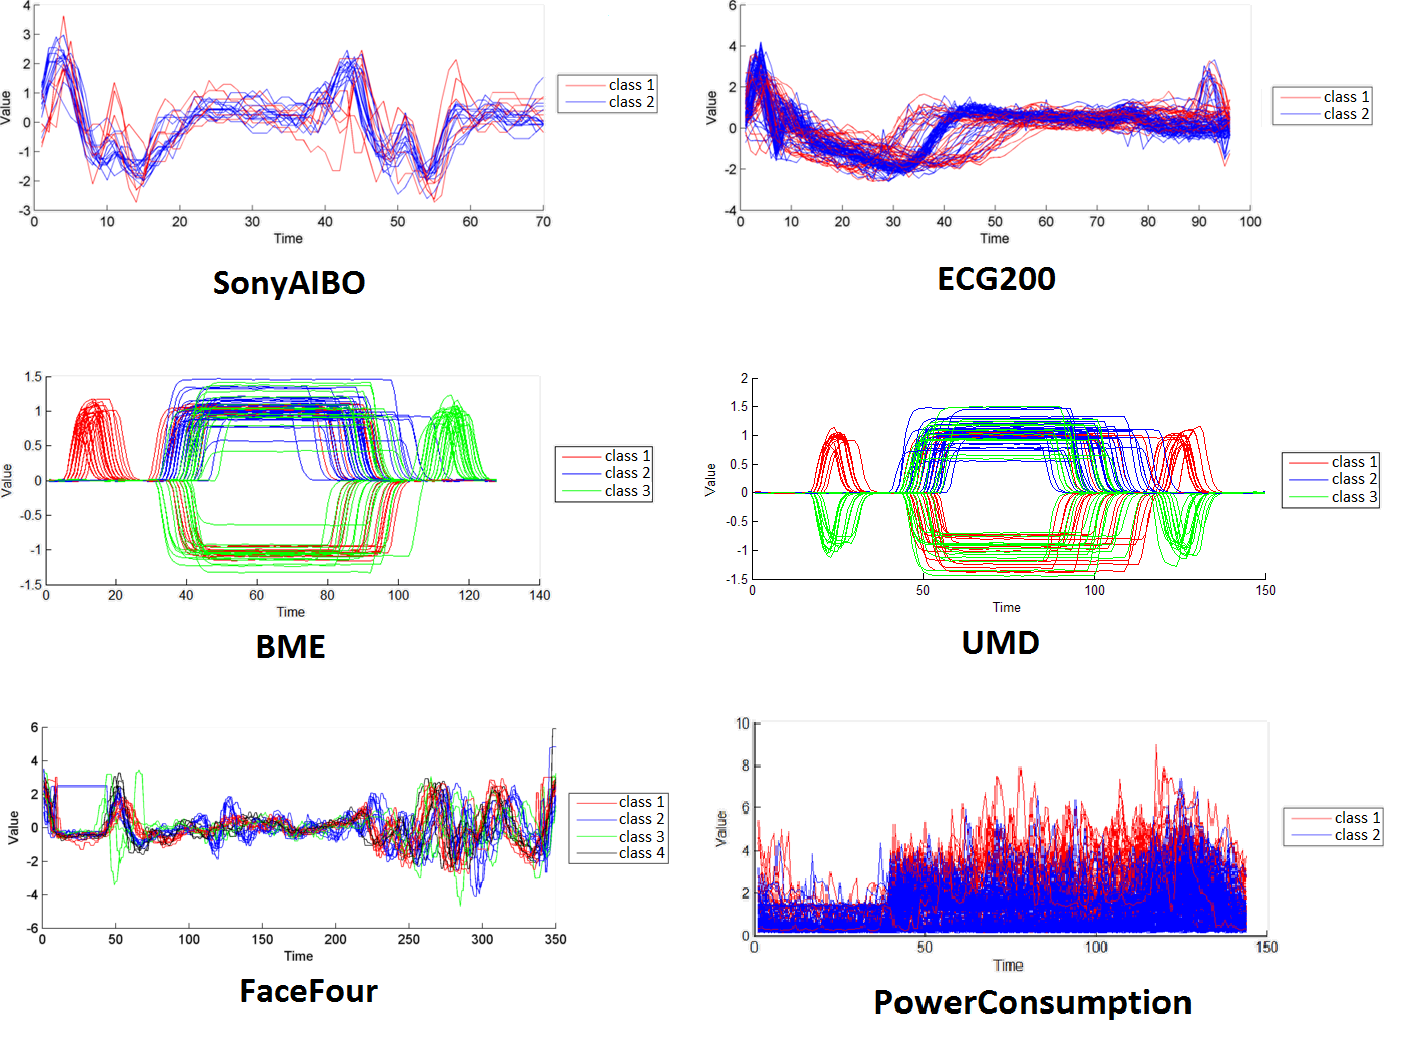
\includegraphics[width=0.85\linewidth]{images/dataset_exp}
	\caption{Temporal representation of some datasets (SonyAIBO, ECG200, BME, UMD, FaceFour, PowerConsumption) considered in our experiments.}
	\label{fig:dataset}
\end{figure}

\newpage
%-----------------------------------------------------------------------------
\section{Experimental protocol}
The combined metrics  $D$ and $D_{\mathcal{H}}$  ($K$ as the Gaussian kernel) are learned under $L_1$ and $L_2$ regularization, respectively. The parameters are estimated on a validation set by line/grid search.  A cross-validation and  stratified sampling for unbalanced datasets are used (Section \ref{sec:model_selection}).  Particularly, for each  couple ($r$, $\lambda$) $r \in \{1, 4, 10\}$ and $\lambda \in \{0, 10, 30\}$, the pairwise {\sc svm} parameters ($C,\alpha, \gamma$) are learned by grid search as indicated in Table \ref{tab:param}. The temporal order $r$ is noise-dependent,  typically 1  is retained for noise-free data. The parameter $\lambda$ corresponds to the strength of the '{\it push'} term; precisely, if  no, moderate or  strong '{\it push}'  is required during the training process, a $\lambda$ value of  0, 10 and 30 is learned, respectively.

\noindent The parameters retained are those that:
\begin{itemize}
	\item \textbf{First}, minimize the average classification error $Err$ on  the validation set (Section \ref{sec:model_selection} \& Section \ref{sec:ClassificationEvaluation}).
	\item \textbf{Secondly}, in the case of multiple solutions ($C,\alpha, \gamma$)  leading to equal performances, the most discriminant one is retained (i.e. making closer positive pairs and far a way negative pairs). Precisely, it minimizes the ratio $\frac{d_{intra}}{d_{inter}}$ where $d_{intra}$ and $d_{inter}$ stands respectively to the mean of all intraclass and interclass distances according to the considered metric $D$ or $D_{\mathcal{H}}$.
\end{itemize} 

\begin{table}[h!]
	\small
	\centering
	\renewcommand{\arraystretch}{0.85}
	\resizebox{0.6\textwidth}{!}{
		\setlength{\tabcolsep}{1pt}
		\begin{tabular}{lcc}
			\hline
			& Parameter & Ranges \\
			\hline
			$d_{B}$                 & $r$       & $\{1, 2, 3, , ..., T-1\}$ \\
			$D$, $D_{\mathcal{H}}$  & $\lambda$ & $\{0, 10, 30\}$ \\
			$D$, $D_{\mathcal{H}}$  & $C$       & $\{10^{-3}, 0.5, 1, 5, 10, 20, 30, ..., 150\}$ \\
			$D$, $D_{\mathcal{H}}$  & $\alpha$  & $\{1,2,3\}$     \\
			$D_{\mathcal{H}}$       & $\gamma$  & $\{10^{-3}, 10^{-2}, ..., 10^{3}\}$ \\
			\hline
		\end{tabular}}
		\caption{Parameter ranges}
		\label{tab:param}
\end{table}
	
%-----------------------------------------------------------------------------
\section{Results}
\begin{table}[h!]
	\small
	\centering
	\renewcommand{\arraystretch}{0.8}
	\resizebox{0.9\textwidth}{!}{
		\setlength{\tabcolsep}{1pt}
		\begin{tabular}{|l|ccccc|ccc|}
			\hline
			& \multicolumn{5}{c|}{Alternative uni-modal metrics} & \multicolumn{2}{c}{{\sc m}$^2${\sc tml}} & {\sc warp}  \\
			\cline{2-9} 
			Dataset & $d_A$ & $d_B$ & $d_F$ & $\mbox{\sc dtw}$ & $d_{B-\mbox{\sc dtw}}$ & $D (\lambda^*)$ & $D_{\mathcal{H}} (\lambda^*)$ & {\sc warp}  \\
			\hline
			1 CC                  & 0.120 & 0.113 & 0.383 & \textbf{0.007} & 0.027     & \textbf{0.003} (0) & \textbf{0.007} (0) & \checkmark \\
			2 GunPoint            & 0.087 & 0.113 & \textbf{0.027} & 0.093 & \textbf{0.027}     & \textbf{0.020} (10) & \textbf{0.040} (10) & \checkmark \\
			3 CBF                 & 0.148 & 0.140 & 0.382 & \textbf{0.003} & \textbf{0.000}        & 0.031 (30) & \textbf{0.003} (0)  & \checkmark \\
			4 OSULeaf             & 0.484 & 0.475 & 0.426 & 0.409 & \textbf{0.265}    & 0.380 (0)  & 0.376 (0)  & \checkmark \\
			5 SwedishLeaf         & 0.211 & 0.186 & 0.146 & 0.208 & \textbf{0.109} & \textbf{0.110} (0) & \textbf{0.114} (0) & \checkmark \\
			6 Trace               & 0.240 & 0.240 & 0.140 & \textbf{0.000}    & \textbf{0.000}        & \textbf{0.000} (0)    & \textbf{0.010} (0)  & \checkmark \\
			7 FaceFour            & 0.216 & 0.216 & 0.239 & 0.170 & 0.136     & \textbf{0.000} (0)     & 0.034 (0)  & \checkmark \\
			8 Lighting2           & \textbf{0.246} & \textbf{0.246} & \textbf{0.148} & \textbf{0.131}& \textbf{0.213}     & \textbf{0.148} (0)  & \textbf{0.131} (0) & \checkmark \\
			9 Lighting7           & 0.425 & 0.411 & \textbf{0.316} & \textbf{0.274} & \textbf{0.288}     & 0.397 (0)  & \textbf{0.233} (0) & \checkmark \\
			10 ECG200              & \textbf{0.120} & \textbf{0.070}& 0.160 & 0.230& 0.190    & \textbf{0.080} (0)  & \textbf{0.080} (0) & $\times$  \\
			11 Adiac               & 0.389 & \textbf{0.297} & \textbf{0.261} & 0.396 & 0.338     & 0.358 (0)  & 0.361 (0) & $\times$\\
			12 FISH                & 0.217 & \textbf{0.149} & 0.229 & \textbf{0.166} & \textbf{0.137}   & \textbf{0.149} (0)  & 0.240 (0) & \checkmark  \\
			13 Beef                & 0.467 & 0.300 & 0.500 & 0.500 & 0.500     & \textbf{0.033} (0) & 0.267 (0) & $\times$   \\
			14 Coffee              & 0.250 & \textbf{0.000}    & 0.357 & 0.179 & 0.143     & \textbf{0.000} (0)     & \textbf{0.000} (10) &$\times$  \\
			15 OliveOil            & \textbf{0.133} & \textbf{0.133} & \textbf{0.167} & \textbf{0.200} & \textbf{0.100}    & \textbf{0.167} (0)  & \textbf{0.100} (10) & \checkmark \\
			16 CinCECGtorso        & 0.103 & 0.367 & 0.167 & 0.349 & 0.367  & \textbf{0.092} (0)  & \textbf{0.079} (0) & $\times$   \\
			17 DiatomSizeR     	& 0.065 & 0.076 & 0.069 & \textbf{0.033} & \textbf{0.029}     & \textbf{0.026} (0)  & \textbf{0.029} (0) & \checkmark \\
			18 ECG5Days            & 0.203 & 0.153 & \textbf{0.006} & 0.232 & 0.236    & \textbf{0.007} (10) & 0.024 (0)  & $\times$   \\
			19 FacesUCR            & 0.231 & 0.227 & 0.175 & 0.095 & 0.102     & \textbf{0.068}  (10) & \textbf{0.059} (0) & \checkmark \\
			20 InlineSkate         & \textbf{0.658} & \textbf{0.658} & 0.675 & \textbf{0.616} & \textbf{0.623}     & 0.733  (10) & \textbf{0.625} (0) & \checkmark \\
			21 ItalyPowerD     	& 0.045 & \textbf{0.028}& 0.078 & 0.050 & 0.055    & \textbf{0.028} (30) & \textbf{0.037} (10) & $\times$  \\
			22 MedicalImages       & 0.316 & 0.313 & 0.345 & \textbf{0.263} & 0.290     & \textbf{0.237} (0) & \textbf{0.236} (10) & \checkmark \\
			23 MoteStrain          & \textbf{0.121} & 0.263& 0.278 & 0.165& 0.171     & 0.185 (0)  & 0.153 (10) & \checkmark \\
			24 SonyAIBOII          & \textbf{0.141} & \textbf{0.142} & \textbf{0.128} & 0.169 & 0.194     & \textbf{0.155} (0)  & \textbf{0.131} (0) & $\times$  \\
			25 SonyAIBO            & 0.305 & 0.308 & 0.258 & 0.275 & 0.343     & \textbf{0.188} (0)  & \textbf{0.165} (30) & $\times$   \\
			26 Symbols             & 0.101 & 0.111 & 0.080 & \textbf{0.050} & \textbf{0.043}     & \textbf{0.034} (30) & \textbf{0.046} (30) & \checkmark \\
			27 TwoLeadECG          & 0.253 & 0.153 & 0.103 & 0.096 & \textbf{0.008}   & \textbf{0.006} (0)  & \textbf{0.016} (10) & \checkmark \\
			28 PowerCons           & \textbf{0.366} & 0.445 & \textbf{0.315} & 0.397 & 0.401     & \textbf{0.318} (0)  & \textbf{0.308} (0) & \checkmark \\
			29 BME 				& 0.173 & 0.180 & 0.373 & 0.107 & 0.120     & \textbf{0.040} (30) & \textbf{0.000} (10) 	     & \checkmark \\
			30 UMD 				& 0.194 & 0.222 & 0.299 & 0.118 & \textbf{0.090}     & 0.104  (0)     & \textbf{0.042} (0) & \checkmark \\ 
			\hline
		\end{tabular}
	}
	\caption{1-NN  error rates for standard and {\sc m}$^2${\sc tml} measures.}
	\label{tab-resu}
\end{table}
%\vspace{-1cm}
Table \ref{tab-resu} reports the  1-NN classification test errors for uni-modal and {\sc m}$^2${\sc tml} metrics; the results that are  statistically and significantly better than the rest are indicated in bold (z-test at  5\% risk detailed in Section \ref{sec:ClassificationEvaluation}). In particular, we compare the $1$-NN error rates when based on uni-modal metrics  (first 5 columns) and on  $D$ and $D_{\mathcal{H}}$. The last column '{\sc warp}' indicates the synchronous (\checkmark) or asynchronous ($\times$) data type. 


%-----------------------------------------------------------------------------
\section{Discussion}
From Table \ref{tab-resu}, we can see first that the 1-NN classification reaches  the best results in: 
\begin{enumerate}
	\item Less than one-third of the data when based on $d_A$, $d_B$ or $d_F$ 
	\item Slightly more than one-third for  $\mbox{\sc dtw}$ and $d_{B-\mbox{\sc dtw}}$ 
	\item More than two-thirds (23 times on 30)  when based on  $D$ or  $D_{\mathcal{H}}$.
\end{enumerate}
% i) less than one-third of the data when based on $d_A$, $d_B$ or $d_F$, ii) slightly more than one-third for  $\mbox{\sc dtw}$ and $d_{B-\mbox{\sc dtw}}$ and iii) more than two-thirds (23 times on 30)  when based on  $D$ or  $D_{\mathcal{H}}$.
Particularly, note that for nearly all datasets for which an uni-modal metric succeeds,  the {\sc m}$^2${\sc tml} metrics succeed similarly or lead to equivalent results.  
However, for  several challenging datasets ({\it e.g.} FaceFour, Beef, FaceUCR, SonyAIBO, BME) {\sc m}$^2${\sc tml} realizes drastic improvements, to the best of our knowledge never achieved before  for these challenging public data. For instance, the impressive scores of 3\% obtained for Beef against an  error rate  varying from 30\% to 50\% for alternative metrics,   and of 0\% obtained for FaceFour  v.s. 13\% to 23\% for alternative metrics.  Finally, $D$ and $D_{\mathcal{H}}$ are all the more outperforming if only compared to the standard metrics $d_A$ (the Euclidean distance) and {\sc dtw}. \\
Thanks to the $L_1$ regularization, the learned {\sc svm} reveals  the features that most differentiate positive from negative pairs.  Table \ref{tab-feature} shows the sparse, muti-modal and multi-scale potential of {\sc m}$^2${\sc tml} approach.  It gives for each dataset, the weights of the top five 'discriminative' features that contribute to the definition of $D$.  For instance,   for FaceFour $D$ reaches the 0\% by combining, in the order of importance, the behavior,  frequential and amplitude modalities, at the global ($I^0$) and  local ($I^4$, $I^5$, $I^2$) scales. For Beef, besides the impressive error rate of 3\%, the learned model is very sparse as $D$ involves only the behavior modality based on   the segment $I^3$ ($d_B^3$). Similarly for Coffee, the obtained 0\% involves  only the behavior and frequential modalities at several scales. \\ 
In Fig.  \ref{fig:w} we plot the  the weights  of all features for SonyAIBO case as an example, that illustrates  the sparsity of the {\sc m}$^2${\sc tml} approach. In summary, we can  emphasize  that for almost all datasets, the definition of  $D$ involves no more than five features (the most contributive ones), that  assesses not only the model's sparsity but also  the representativeness of the revealed features.
\begin{table}[h!]
	%	\small
	\centering
	\renewcommand{\arraystretch}{1.3}
	\resizebox{1\textwidth}{!}{
		\setlength{\tabcolsep}{1pt}
		\begin{tabular}{| c |  l l l l l |}
			\hline
			Dataset & \multicolumn{5}{c|}{Feature weights  (\%)}  \\ 
			\hline 
			%\vspace{0.1cm}
			CC					& {\sc dtw}$^2$ (56.3\%)&   $d_F^0$ (18.8\%)&   $d_F^4$ (5.9\%)&   $d_F^1$ (4\%)&   $d_{B-\mbox{\sc dtw}}^0$ (3.2\%)
			\\
			GunPoint			& $d_{B-\mbox{\sc dtw}}^0$ (42.1\%)&   {\sc dtw}$^5$ (10.9\%)&   {\sc dtw}$^1$ (10.2\%)&   $d_{B-\mbox{\sc dtw}}^6$ (8.4\%)&   $d_F^4$ (8.1\%) 
			\\
			CBF 				& {\sc dtw}$^4$ (56.5\%)&   $d_F^3$ (43.4\%)&   $d_{B-\mbox{\sc dtw}}^1$ (0.2\%)&   {\sc dtw}$^0$ (0\%)&   $d_{B-\mbox{\sc dtw}}^0$ (0\%)
			\\
			OSULeaf				& {\sc dtw}$^2$ (23.7\%)&   $d_F^0$ (19.5\%)&   $d_{B-\mbox{\sc dtw}}^0$ (14.6\%)&   $d_{B-\mbox{\sc dtw}}^2$ (9.4\%)&   {\sc dtw}$^1$ (9\%)   
			\\
			SwedishLeaf			& $d_F^0$ (21.5\%)&   {\sc dtw}$^0$ (15.9\%)&   $d_{B-\mbox{\sc dtw}}^0$ (15.2\%)&   {\sc dtw}$^6$ (11.5\%)&   $d_{B-\mbox{\sc dtw}}^1$ (6.1\%)   
			\\
			Trace 				& {\sc dtw}$^0$ (58.3\%)&   {\sc dtw}$^6$ (6.9\%)&   $d_{B-\mbox{\sc dtw}}^0$ (5.8\%)&   {\sc dtw}$^2$ (5.6\%)&   {\sc dtw}$^5$ (5.5\%) 
			\\
			FaceFour			& $d_{B-\mbox{\sc dtw}}^4$ (44.5\%)&   $d_F^4$ (12.7\%)&   {\sc dtw}$^5$ (11.1\%)&   {\sc dtw}$^0$ (8.3\%)&   {\sc dtw}$^2$ (6.4\%)   
			\\
			Lighting2			& $d_{B-\mbox{\sc dtw}}^0$ (30.4\%)&   {\sc dtw}$^6$ (18.7\%)&   $d_F^1$ (16.5\%)&   $d_{B-\mbox{\sc dtw}}^6$ (13.4\%)&   {\sc dtw}$^0$ (10.7\%)  
			\\
			Lighting7			& $d_{B-\mbox{\sc dtw}}^6$ (87.4\%)&   $d_F^6$ (8.6\%)&   $d_{B-\mbox{\sc dtw}}^5$ (4\%)  & -  & - 
			\\
			ECG200				& $d_B^0$ (89.6\%)&   $d_B^6$ (2.4\%)&   $d_A^3$ (2.3\%)&   $d_B^1$ (2.2\%)&   $d_B^4$ (2\%)  
			\\
			Adiac				& $d_F^0$ (79.2\%)&   $d_B^4$ (13.8\%)&   $d_A^4$ (3.5\%)&   $d_F^5$ (1.7\%)&   $d_B^5$ (1.2\%)   
			\\
			FISH				& $d_{B-\mbox{\sc dtw}}^5$ (17.9\%)&   $d_F^0$ (10.5\%)&   $d_{B-\mbox{\sc dtw}}^6$ (9.9\%)&   $d_{B-\mbox{\sc dtw}}^4$ (8.3\%)&   $d_{B-\mbox{\sc dtw}}^3$ (7.8\%)  
			\\
			Beef				& $d_B^3$ (100\%)& - & - &-  & -  
			\\
			Coffee				& $d_B^2$ (22.4\%)&   $d_F^4$ (20.1\%)&   $d_B^6$ (14.6\%)&   $d_B^0$ (8.1\%)&   $d_F^5$ (7\%)   
			\\
			OliveOil			& $d_F^5$ (97\%)&   $d_{B-\mbox{\sc dtw}}^2$ (3\%)   & - & - & -
			\\
			CinCECGtorso		& $d_F^0$ (38.4\%)&   $d_A^5$ (13.1\%)&   $d_B^4$ (11.5\%)&   $d_F^1$ (11.2\%)&   $d_A^2$ (9.8\%)   
			\\
			DiatomSizeR 		& $d_F^5$ (39.1\%)&   $d_F^0$ (36\%)&   $d_{B-\mbox{\sc dtw}}^4$ (24.9\%)  & - & - 
			\\
			ECG5Days			& $d_B^5$ (59.5\%)&   $d_B^6$ (32.3\%)&   $d_A^4$ (3.9\%)&   $d_B^2$ (3.1\%)&   $d_B^4$ (1.2\%)  
			\\
			FacesUCR			& $d_F^2$ (21.5\%)&   $d_{B-\mbox{\sc dtw}}^0$ (19.5\%)&   $d_F^4$ (16.7\%)&   {\sc dtw}$^0$ (12.6\%)&   $d_{B-\mbox{\sc dtw}}^2$ (8.6\%)
			\\
			InlineSkate			& $d_F^4$ (42.5\%)&   {\sc dtw}$^5$ (22.8\%)&   {\sc dtw}$^4$ (17.6\%)&   {\sc dtw}$^2$ (6.7\%)&   $d_{B-\mbox{\sc dtw}}^6$ (5.9\%)   
			\\
			ItalyPowerD 		& $d_B^6$ (68.7\%)&   $d_B^0$ (25.9\%)&   $d_B^3$ (5.2\%)&   $d_B^4$ (0.2\%)   & -
			\\
			MedicalImages		& $d_{B-\mbox{\sc dtw}}^1$ (53.3\%)&   $d_F^3$ (12.9\%)&   $d_{B-\mbox{\sc dtw}}^2$ (10.7\%)&   $d_{B-\mbox{\sc dtw}}^3$ (10.1\%)&   $d_{B-\mbox{\sc dtw}}^0$ (3.8\%)   
			\\
			MoteStrain			& $d_{B-\mbox{\sc dtw}}^5$ (93.2\%)&   $d_{B-\mbox{\sc dtw}}^6$ (6.8\%)& -  & - & -
			\\
			SonyAIBOII			& $d_B^3$ (100\%)& -   & - & - &- 
			\\
			SonyAIBO			& $d_F^3$ (30.8\%)&   $d_B^6$ (27.3\%)&   $d_B^5$ (5\%)&   $d_A^1$ (4.1\%)&   $d_B^0$ (3.9\%)   
			\\
			Symbols 			& $d_{B-\mbox{\sc dtw}}^0$ (45.6\%)&   $d_{B-\mbox{\sc dtw}}^6$ (35.3\%)&   $d_{B-\mbox{\sc dtw}}^5$ (19\%)&   {\sc dtw}$^0$ (0.1\%)   & -
			\\
			TwoLeadECG 			& $d_{B-\mbox{\sc dtw}}^4$ (60\%)&   $d_F^1$ (12\%)&   {\sc dtw}$^4$ (11.4\%)&   $d_{B-\mbox{\sc dtw}}^6$ (7.6\%)&   $d_{B-\mbox{\sc dtw}}^1$ (4.2\%)
			\\
			PowerCons			& $d_F^0$ (26.1\%)&   {\sc dtw}$^0$ (20.3\%)&   $d_F^1$ (19.3\%)&   $d_{B-\mbox{\sc dtw}}^0$ (6.1\%)&   $d_F^2$ (5.1\%) 
			\\
			BME 				& $d_{B-\mbox{\sc dtw}}^0$ (75.2\%)&   $d_F^4$ (15.5\%)&   $d_{B-\mbox{\sc dtw}}^2$ (5.8\%)&   $d_{B-\mbox{\sc dtw}}^1$ (1.9\%)&   $d_F^1$ (0.7\%)   
			\\
			UMD 				& $d_{B-\mbox{\sc dtw}}^0$ (99.8\%)&   $d_{B-\mbox{\sc dtw}}^5$ (0.2\%)& -& -& -  \\
			\hline
		\end{tabular}
	}
	\caption{Top 5  multi-modal and multi-scale features involved in  $D$}
	\label{tab-feature}
\end{table}

\begin{figure}[h!]
	\centering
	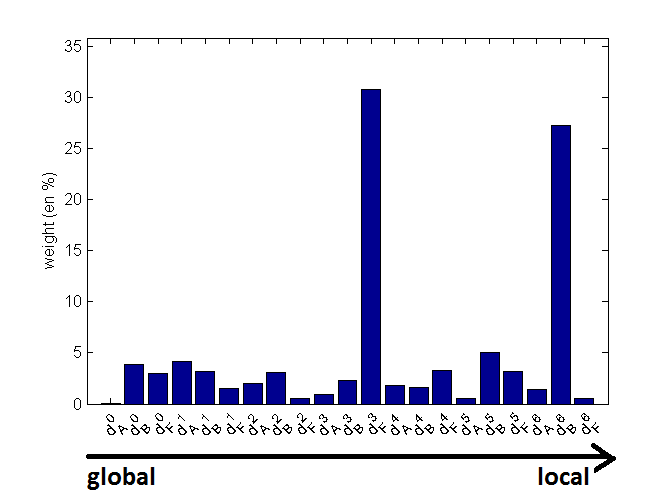
\includegraphics[width=0.6\linewidth]{images/SonyAIBO_weight_V2}
	\caption{SonyAIBO:  {\sc m}$^2${\sc tml} feature weights}
	\label{fig:w}
\end{figure}

In the second part,  we perform a graphical analysis for a global comparison on the whole datasets.  In Fig. \ref{fig:error1},  each dataset is projected according to, on the x-axis its best error rate obtained for $D$ and  $D_{\mathcal{H}}$, and on y-axis  its best performance w.r.t  the standard metrics $d_A$  and  {\sc dtw}. In Fig. \ref{fig:error2},  the y-axis is related to the best error rate w.r.t {\sc dtw} and $d_{B-\mbox{\sc dtw}}$, the two most performant uni-modal metrics. For both plots we can note that the datasets are principally  projected above the first bisector, indicating higher error rates mostly obtained for alternative metrics than for {\sc m}$^2${\sc tml}. For the less challenging datasets, although almost projected near the bisector denoting equal performances for the compared metrics, {\sc m}$^2${\sc tml}  still  bring improvements with projections clearly positioned  above the bisector.  Finally, from Fig. \ref{fig:error2} we can see that {\sc m}$^2${\sc tml} metrics perform significantly lower than $d_{B-\mbox{\sc dtw}}$ on OSUleaf, while InlineSkate dataset remains challenging for all studied metrics.
\begin{figure}[h!]
	\centering
	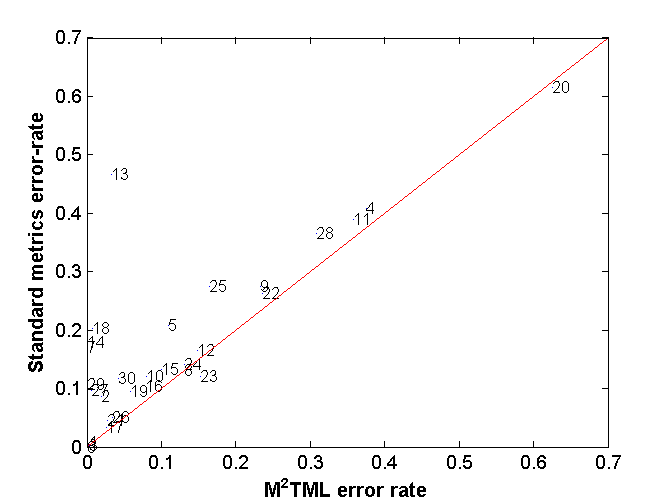
\includegraphics[width=0.6\linewidth]{images/Stand_m2tml}
	\caption{Standard (Euclidean distance $d_A$  and {\sc dtw}) {\it vs.} {\sc m}$^2${\sc tml} ($D$ and $D_{\mathcal{H}}$) metrics }
	\label{fig:error1}
\end{figure}
\begin{figure}[h!]
	\centering
	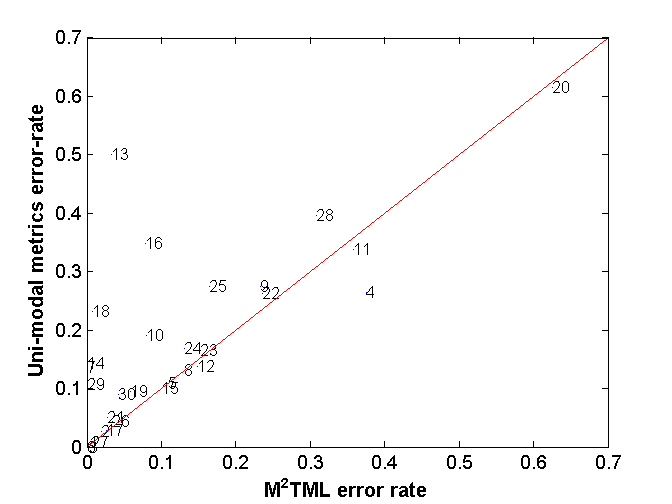
\includegraphics[width=0.6\linewidth]{images/Unimod_m2tml}
	\caption{Best Uni-modal ({\sc dtw} and $d_{B-\mbox{\sc dtw}}$) {\it vs.} {\sc m}$^2${\sc tml} ($D$  and $D_{\mathcal{H}}$) metrics }
	\label{fig:error2}
\end{figure}


In the last part we compare the global effect of the alternative and {\sc m}$^2${\sc tml} metrics  on the 1-NN neighborhood distribution and class discrimination. For that, an  {\sc mds}\footnote{matlab function: mdscale for metrics and non metrics} is used to vizualize  the distribution of samples according to their pairwise  dissimilarities.
For instance, for FaceFour, Fig. \ref{fig:mds} shows the first obtained plans and their corresponding stresses, the classes being indicated in different symbols and colors. We can see distinctly the effect of the learned  $D$ that leads to  more compact and more isolated classes with  robust  neighborhoods for 1-NN classification ({\it i.e.} closer positive pairs and far away negative pairs) than  the best alternative metric $d_{B-\mbox{\sc dtw}}$ that shows more overlapping classes and heterogeneous neighborhoods.
\begin{figure}[h!]
	\centering
	% 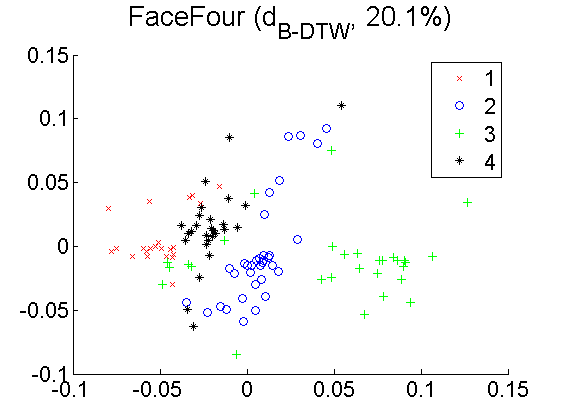
\includegraphics[width=0.6\linewidth]{images/FaceFourALL_DTWDB_1} \hspace{-0.45cm}
	% 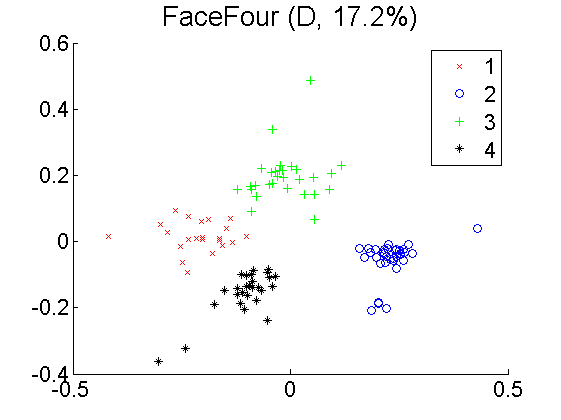
\includegraphics[width=0.6\linewidth]{images/FaceFourALL_D_Delay_1}
	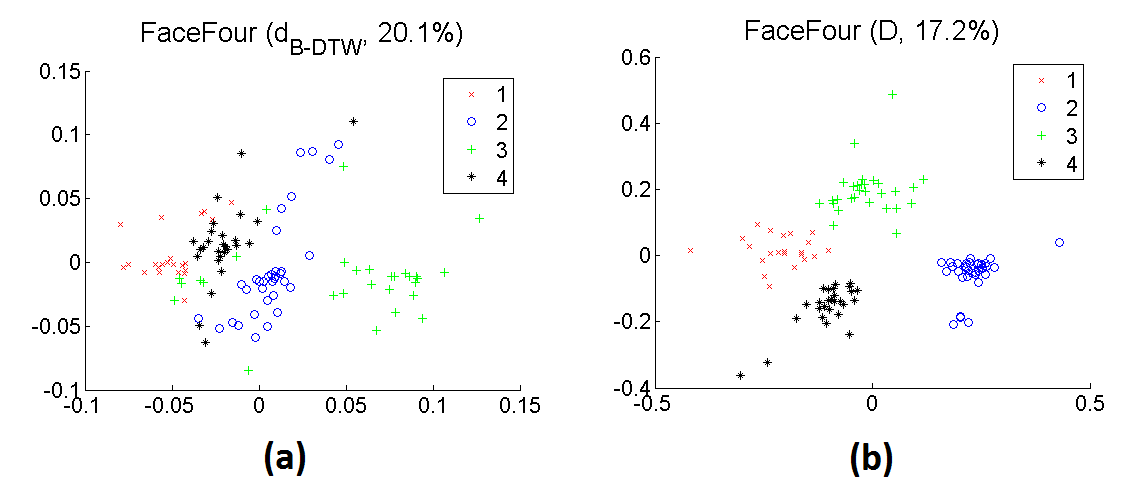
\includegraphics[width=1\linewidth]{images/FaceFour}
	\caption{{\sc mds} visualization of the $d_{B-\mbox{\sc dtw}}$ (left) and $D$ (right) dissimilarities for FaceFour data}
	\label{fig:mds}
\end{figure} 

\newpage
\section{Conclusion of the chapter}
%%% Local Variables: 
%%% mode: latex
%%% TeX-master: "../roque-phdthesis"
%%% End: 
